\documentclass{standalone}

\usepackage{tikz}
\usetikzlibrary{positioning, arrows.meta, decorations.pathmorphing}

\begin{document}
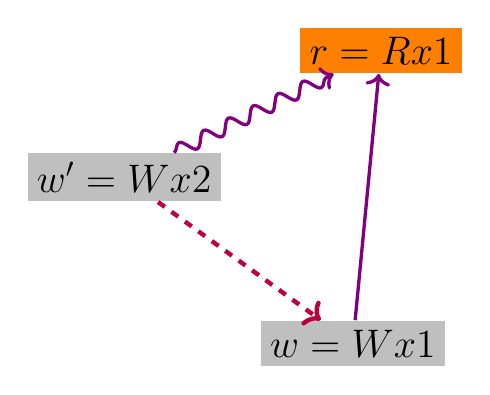
\begin{tikzpicture}[read/.style = {fill = orange, font = \Large},
  write/.style = {fill = lightgray, font = \Large},
  rwmap/.style = {->, violet, very thick},
  reach/.style = {->, violet, very thick, decorate, decoration = snake},
  wprimew/.style = {->, purple, dashed, ultra thick}]

  \node(wprime) [write] {$w' = Wx2$};
  \node(w) [write, below right = 1.5cm and 0.5cm of wprime] {$w = Wx1$};
  \node(r) [read, above right = of wprime] {$r = Rx1$};

  \draw[rwmap] (w) to (r);
  \draw[reach] (wprime) to (r);
  \draw[wprimew] (wprime) to (w);
\end{tikzpicture}
\end{document}
